% !Mode:: "TeX:UTF-8"
% Author: Zhengxi Tian
% Email: zhengxi.tian@hotmail.com

\chapter{实验结果与讨论}\label{ch:experiment}
本章从系统层面得分,句子层面得分和定性分析三个方面展示了实验的数据与结论。

\section{系统层面得分}\label{sec:system_scores}
图~\ref{tab:systemScoresAll}~展示了各个模型在不同数据集上测定的各种指标的系统层面得分,
加粗的得分是三个系统中的最优者。
从表中的数据来看,在LSDSCC上的最优模型是HRED,
在OpenSubtitles上的最优模型是VHRED,
在Ubuntu上的最优模型是HRED,它在9个指标中取得了最优,但是LSTM也在6个指标中取得了最优。

\begin{table}%
\centering%
\caption{不同数据集上的模型的各种指标得分}%
\label{tab:systemScoresAll}%
\begin{tabular}{|l|l|l|l|l|l|l|l|l|l|}%
\hline%
&\multicolumn{3}{c|}{LSDSCC}&\multicolumn{3}{c|}{OpenSubtitles}&\multicolumn{3}{c|}{Ubuntu}\\%
\hline%
&HRED&LSTM&VHRED&HRED&LSTM&VHRED&HRED&LSTM&VHRED\\%
\hline%
ADEM&2.6178&2.6127&2.6163&2.6228&2.6224&2.6219&2.6353&2.6381&2.635\\%
\hline%
BLEU{-}1&0.08&0.0726&0.0722&0.0672&0.0638&0.0753&0.1314&0.1303&0.1365\\%
\hline%
BLEU{-}2&0.0264&0.0181&0.0185&0.0171&0.0153&0.0264&0.0362&0.0345&0.0375\\%
\hline%
BLEU{-}3&0.0105&0.0052&0.0066&0.0062&0.0055&0.0146&0.009&0.007&0.0089\\%
\hline%
BLEU{-}4&0.0053&0.0&0.0028&0.0024&0.0022&0.01&0.0029&0.0018&0.0025\\%
\hline%
Distinct{-}1&0.9577&0.9441&0.9558&0.973&0.9714&0.9714&0.9074&0.9257&0.9113\\%
\hline%
Distinct{-}2&0.8541&0.8511&0.8497&0.8669&0.8594&0.8665&0.9013&0.8603&0.8968\\%
\hline%
Greedy&0.3303&0.3292&0.3267&0.3102&0.2998&0.3145&0.2775&0.2364&0.273\\%
\hline%
Average&0.5532&0.5467&0.5483&0.5453&0.5295&0.5485&0.574&0.5205&0.5655\\%
\hline%
Extrema&0.2841&0.2835&0.2814&0.3009&0.2929&0.3061&0.29&0.2663&0.2875\\%
\hline%
METEOR&0.0296&0.0258&0.0281&0.0248&0.0233&0.0271&0.1657&0.1635&0.166\\%
\hline%
ROUGE{-}1&0.108&0.083&0.0978&0.0784&0.075&0.0872&0.1644&0.1836&0.1683\\%
\hline%
ROUGE{-}2&0.0226&0.0049&0.0081&0.0053&0.0043&0.0107&0.0128&0.0143&0.0128\\%
\hline%
ROUGE{-}3&0.0057&0.0002&0.0035&0.0011&0.0009&0.0053&0.0007&0.0003&0.0005\\%
\hline%
ROUGE{-}4&0.0011&0.0&0.003&0.0002&0.0002&0.0038&0.0002&0.0&0.0001\\%
\hline%
ROUGE{-}L&0.0956&0.0681&0.0846&0.0742&0.0707&0.0826&0.1493&0.1722&0.1535\\%
\hline%
ROUGE{-}W&0.0792&0.0537&0.07&0.066&0.0629&0.0734&0.1205&0.1391&0.1236\\%
\hline%
PPL&32.5599&32.9229&37.7149&41.6392&34.2724&33.6867&39.178&46.4061&40.2641\\%
\hline%
\#words&13.1605&14.0067&12.3612&8.807&8.6394&8.7798&23.0646&16.4905&21.2449\\%
\hline%
\end{tabular}%
\end{table}

\section{句子层面得分}\label{sec:utterance_scores}
我们还从句子层面得分方面进行了分析。
因为模型生成的句子$u$可以看做一个句子空间$U$上的随机变量,而指标是一个确定的函数$f_{s}$,
所以可以把句子层面的得分看做一个随机变量$\lambda_u = f_{s}(u)$。
于是我们便可以用概率分布的工具来分析指标在句子水平的情况。

\subsection{指标的概率分布}\label{subsec:metric_distribution}
我们首先观察了各种指标的句子层面得分的单变量分布(Univariate Distribution)。
为了突出普遍性,我们首先对每个指标绘制了在所有模型和数据集的组合上的概率分布图。
为了便于从图像上比较各种指标的分布特征,我们对数值作了正则化处理,使数据的平均值为0,标准为1:
\begin{align}
    x' = \frac{x - \mu}{\sigma}
\end{align}
中心极限定理表明(Central Limit Theorems):大量独立随机变量的叠加近似于高斯分布。
因为各位人类评价员之间的评价是独立的, 我们假设当句子足够多时,句子层面的人类评价近似于高斯分布。
从该假设出发可以认为,句子层面得分的分布接近高斯分布是一个指标和人类评价具有较高相关性的前提条件。

如图~\ref{fig:ADEMdist}~所示,ADEM的分布非常接近高斯分布(Gaussian Distribution),
并且ADEM与人类评价的相关性比较高\upcite{ADEM}。
\begin{figure}[H]%
\centering%
\includegraphics[width=0.8\textwidth]{/home/cgsdfc/Metrics/Eval/data/v2/plot/distplot_grid/adem/plot.pdf}%
\caption{ADEM 的概率分布图}%
\label{fig:ADEMdist}%
\end{figure}

% -- bleu -- %
\begin{figure}[H]%
\centering%
\includegraphics[width=0.6\textwidth]{/home/cgsdfc/Metrics/Eval/data/v2/plot/distplot_grid/bleu_1/plot.pdf}%
\caption{BLEU{-}1 的概率分布图}%
\label{fig:BLEU{-}1dist}%
\end{figure}
\begin{figure}[H]%
\centering%
\includegraphics[width=0.6\textwidth]{/home/cgsdfc/Metrics/Eval/data/v2/plot/distplot_grid/bleu_2/plot.pdf}%
\caption{BLEU{-}2 的概率分布图}%
\label{fig:BLEU{-}2dist}%
\end{figure}
\begin{figure}[H]%
\centering%
\includegraphics[width=0.8\textwidth]{/home/cgsdfc/Metrics/Eval/data/v2/plot/distplot_grid/bleu_3/plot.pdf}%
\caption{BLEU{-}3 的概率分布图}%
\label{fig:BLEU{-}3dist}%
\end{figure}
\begin{figure}[H]%
\centering%
\includegraphics[width=0.6\textwidth]{/home/cgsdfc/Metrics/Eval/data/v2/plot/distplot_grid/bleu_4/plot.pdf}%
\caption{BLEU{-}4 的概率分布图}%
\label{fig:BLEU{-}4dist}%
\end{figure}

% -- EB -- %
\begin{figure}[H]%
\centering%
\includegraphics[width=0.6\textwidth]{/home/cgsdfc/Metrics/Eval/data/v2/plot/distplot_grid/embedding_based_greedy_matching/plot.pdf}%
\caption{Greedy 的概率分布图}%
\label{fig:Greedydist}%
\end{figure}
\begin{figure}[H]%
\centering%
\includegraphics[width=0.8\textwidth]{/home/cgsdfc/Metrics/Eval/data/v2/plot/distplot_grid/embedding_based_vector_average/plot.pdf}%
\caption{Average 的概率分布图}%
\label{fig:Averagedist}%
\end{figure}
\begin{figure}[H]%
\centering%
\includegraphics[width=0.6\textwidth]{/home/cgsdfc/Metrics/Eval/data/v2/plot/distplot_grid/embedding_based_vector_extrema/plot.pdf}%
\caption{Extrema 的概率分布图}%
\label{fig:Extremadist}%
\end{figure}

% -- METEOR -- %
\begin{figure}[H]%
\centering%
\includegraphics[width=0.8\textwidth]{/home/cgsdfc/Metrics/Eval/data/v2/plot/distplot_grid/meteor/plot.pdf}%
\caption{METEOR 的概率分布图}%
\label{fig:METEORdist}%
\end{figure}

% -- Distinct-N -- %
\begin{figure}[H]%
\centering%
\includegraphics[width=0.8\textwidth]{/home/cgsdfc/Metrics/Eval/data/v2/plot/distplot_grid/distinct_1/plot.pdf}%
\caption{Distinct{-}1 的概率分布图}%
\label{fig:Distinct{-}1dist}%
\end{figure}
\begin{figure}[H]%
\centering%
\includegraphics[width=0.8\textwidth]{/home/cgsdfc/Metrics/Eval/data/v2/plot/distplot_grid/distinct_2/plot.pdf}%
\caption{Distinct{-}2 的概率分布图}%
\label{fig:Distinct{-}2dist}%
\end{figure}

% -- ROUGE -- %
\begin{figure}[H]%
\centering%
\includegraphics[width=0.6\textwidth]{/home/cgsdfc/Metrics/Eval/data/v2/plot/distplot_grid/rouge_1/plot.pdf}%
\caption{ROUGE{-}1 的概率分布图}%
\label{fig:ROUGE{-}1dist}%
\end{figure}
\begin{figure}[H]%
\centering%
\includegraphics[width=0.8\textwidth]{/home/cgsdfc/Metrics/Eval/data/v2/plot/distplot_grid/rouge_2/plot.pdf}%
\caption{ROUGE{-}2 的概率分布图}%
\label{fig:ROUGE{-}2dist}%
\end{figure}
\begin{figure}[H]%
\centering%
\includegraphics[width=0.8\textwidth]{/home/cgsdfc/Metrics/Eval/data/v2/plot/distplot_grid/rouge_3/plot.pdf}%
\caption{ROUGE{-}3 的概率分布图}%
\label{fig:ROUGE{-}3dist}%
\end{figure}
\begin{figure}[H]%
\centering%
\includegraphics[width=0.8\textwidth]{/home/cgsdfc/Metrics/Eval/data/v2/plot/distplot_grid/rouge_4/plot.pdf}%
\caption{ROUGE{-}4 的概率分布图}%
\label{fig:ROUGE{-}4dist}%
\end{figure}
\begin{figure}[H]%
\centering%
\includegraphics[width=0.6\textwidth]{/home/cgsdfc/Metrics/Eval/data/v2/plot/distplot_grid/rouge_l/plot.pdf}%
\caption{ROUGE{-}L 的概率分布图}%
\label{fig:ROUGE{-}Ldist}%
\end{figure}
\begin{figure}[H]%
\centering%
\includegraphics[width=0.6\textwidth]{/home/cgsdfc/Metrics/Eval/data/v2/plot/distplot_grid/rouge_w/plot.pdf}%
\caption{ROUGE{-}W 的概率分布图}%
\label{fig:ROUGE{-}Wdist}%
\end{figure}

% -- #words -- %
\begin{figure}[H]%
\centering%
\includegraphics[width=0.6\textwidth]{/home/cgsdfc/Metrics/Eval/data/v2/plot/distplot_grid/utterance_len/plot.pdf}%
\caption{\#words 的概率分布图}%
\label{fig:wordsdist}%
\end{figure}

\subsection{不同指标的相关性分析}\label{subsec:metric_correlation}

\section{定性分析}\label{sec:qualitative_analysis}

\section{结果与讨论}\label{sec:result_and_discussion}

\section{本章小结}\label{sec:experiment_conclusion}
